\documentclass[main.tex]{subfiles}
\begin{document}
\session{01}{12-11-2026}

%=====================================================================
\section{Reading}

Read the first chapter of the CUDA Programming Guide:\\
\url{https://docs.nvidia.com/cuda/cuda-programming-guide/01-introduction/introduction.html}

With focus on:
\begin{itemize}[nosep]
  \item CUDA and the CUDA Programming Guide
  \item 1.1.1.\ The Graphics Processing Unit
  \item 1.1.2.\ The Benefits of Using GPUs
  \item 1.1.3.\ Getting Started Quickly
  \item 1.2.2.1.\ Thread Blocks and Grids
  \item 1.2.2.1.1.\ Thread Block Clusters
  \item 1.2.2.2.\ Warps and SIMT
  \item 1.2.3.4.\ Unified Memory
\end{itemize}

%=====================================================================
\section{Examples: ``hello'' to array flip}

In the following exercises, every new piece of functionality has a comment above it that explains it.

\subsection{01\_hello.cu}
\paragraph{Short version.}
\begin{lstlisting}[language=CUDA]
// description: "Write a .cu file that prints a hello message once from the GPU and once from the CPU."

#include <cstdio>
__global__ void hello(){
    printf("hello from gpu\n");
}
int main(){
    hello<<<1,1>>>();
    cudaDeviceSynchronize();
    printf("hi from cpu\n");
}
\end{lstlisting}
\paragraph{Long version.}
\begin{lstlisting}[language=CUDA]
// <cstdio> is the C standard input/output library (C++ name for stdio.h).
#include <cstdio>

// __global__ marks a kernel: it is CALLED from the CPU but RUNS on the GPU.
// "global" because it is visible to both sides. The only way to run your own code on the GPU is through a kernel. Helpers marked __device__ can then be called from a kernel.
// void is the RETURN TYPE. __global__ is an "execution space specifier".
__global__ void hello() {
    // this printf runs on the GPU and is NOT the stdio one. It has the same name, but writes into a buffer in GPU memory that is copied to the terminal at the next synchronization.
    printf("Hello from the GPU\n");
}

// main() ALWAYS runs on the CPU. Only the body of hello() runs on the GPU.
// In C++ main must return int; e.g. "void main()" is a compile error ('main' must return 'int').
//  main is the only function where you may leave out "return 0;": it then returns 0 automatically. That is why this code has no return.
int main() {
    // Launch the kernel on the GPU: <<<arg 1 =number of blocks, arg 2 = threads per block>>>.
    // " launch the hello kernel with 1 block of 1 thread".
    // Each thread runs the whole body of hello() once, so 1 thread = 1 line of output.
    // hello<<<2, 8>>>() would be 2 blocks of 8 threads = 16 threads which would be 16 times "Hello from the GPU".
    // The launch is asynchronous: the CPU does not wait and continues immediately.
    hello<<<1, 1>>>();

    // cudaDeviceSynchronize() is a CUDA function, called on the CPU, that makes the CPU  wait until the GPU has finished all launched work. It also flushes the GPU's printf output. Then the CPU simply continues with the next line, as it always would. Without it, the program could end before the GPU has printed anything.
    // cudaDeviceSynchronize = wait for the GPU
    cudaDeviceSynchronize();


    // this is the normal C printf from <cstdio>, running on the CPU and writing to the terminal.
    printf("Hello from the CPU\n");
}

// Output:
// Hello from the GPU
// Hello from the CPU
\end{lstlisting}

\subsection{02\_threads.cu}
\paragraph{Short version.}
\begin{lstlisting}[language=CUDA]
//description: Launch 1 block of 8 threads; each thread prints its own index (threadIdx.x) on a new line.

#include <cstdio>

__global__ void hello(){
    printf("current thread %d\n", threadIdx.x);

}
int main(){
    hello<<<1, 8>>>();
    cudaDeviceSynchronize();
}
\end{lstlisting}
\paragraph{Long version.}
\begin{lstlisting}[language=CUDA]
// <cstdio> is included for printf. nvcc would still compile without it, because nvcc automatically includes cuda_runtime.h, which includes stdio.h. Including it is best practice.
#include <cstdio>

__global__ void hello() {
    // threadIdx.x is a built-in variable that exists automatically in every kernel.
    // It is the index of this thread within its block: 0..7 here.
    // Every thread sees a different value; that is how threads tell themselves apart.
    //
    // threads each run this line once, so you get 8 lines, 0 to 7.
    //
    // %d is a placeholder: printf replaces it with the integer argument (threadIdx.x).
    // \n is a newline.
    // (std::cout does not work on the GPU, only printf.)
    //
    // threadIdx is ONE variable, a struct with three fields: threadIdx.x, threadIdx.y, threadIdx.z.
    // (There is no "threadIdy"; it is always threadIdx.something.)
    // With a 1D launch like <<<1, 8>>>, only .x changes; .y and .z are always 0.
    printf("thread %d\n", threadIdx.x);
}

int main() {
    hello<<<1, 8>>>();
    cudaDeviceSynchronize();
}

// Output (order is not guaranteed, but within one block it is usually in order):
// thread 0
// thread 1
// thread 2
// thread 3
// thread 4
// thread 5
// thread 6
// thread 7
//
// Why not guaranteed: all threads run in parallel, and the GPU's hardware scheduler decides which threads execute when. Threads are run in groups of 32 (warps). Within one warp the printf usually comes out in thread order, but CUDA does not promise it. Between warps and between blocks there is no order at all: blocks can run on different parts of the GPU, at the same time, in any order.  never write code that depends on thread order!
\end{lstlisting}
\begin{figure}[H]
\centering
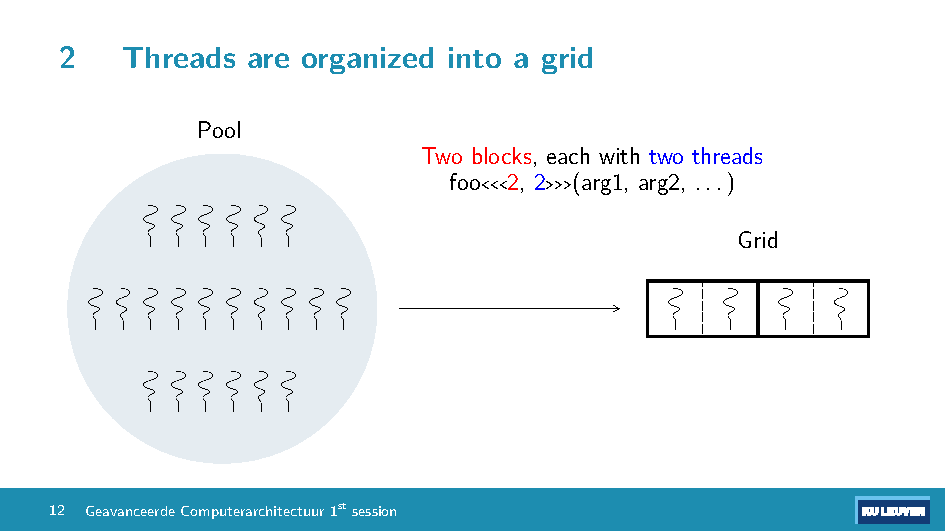
\includegraphics[width=0.72\linewidth, trim=0 20pt 0 0, clip, frame]{figures/session_1_figures/slide-15.pdf}
\caption{Threads are organized into a grid of blocks.}
\end{figure}

\subsection{02b\_threads\_2d.cu (2D thread block / multidimensional thread indexing)}
\paragraph{Short version.}
\begin{lstlisting}[language=CUDA]
//description: Launch 1 block of 4 x 2 threads using dim3; each thread prints its threadIdx.x and threadIdx.y.

#include <cstdio>

__global__ void hello(){
    printf("current threadIdx.x x=%d and threadIdx.y y= %d\n", threadIdx.x, threadIdx.y);
}
int main(){
    dim3 threads(4, 2);
    hello<<<1, threads >>>();
    cudaDeviceSynchronize();
}
\end{lstlisting}
\paragraph{Long version.}
\begin{lstlisting}[language=CUDA]
// Why threadIdx.x or threadIdx.y or threadIdx.z... 2D/3D? It is purely a convenience for the programmer, not a hardware feature.
// The hardware still sees the threads as one long line (x counts fastest, then y, then z)
// and groups them into warps of 32 in that order. Performance is the same.
// The benefit: the indices match the shape of the data.
//   - 2D: images (x = column, y = row), matrices.  3D: volumes (CT scans, voxels, 3D simulations).
//   - Without it you would compute row = i / W and col = i % W yourself; with 2D you get them directly.
// Very common: almost every image or matrix kernel uses 2D blocks, e.g. 16 x 16 threads.
// Every CUDA GPU supports 1D, 2D and 3D blocks and grids (block z is limited to 64).
// Also: x * y * z <= 1024 threads per block in total. dim3(32, 32) = 1024 is the max for a 2D block.
#include <cstdio>

__global__ void hello() {
    // threadIdx and blockIdx are of type uint3, blockDim and gridDim are of type dim3.
    // Now the block is 2D, so every thread has two indices:
    //   threadIdx.x = column inside the block: 0..3
    //   threadIdx.y = row inside the block:    0..1
    printf("thread x=%d y=%d\n", threadIdx.x, threadIdx.y);
}

int main() {
    // dim3 is a CUDA built-in vector type: a small struct with three numbers (x, y, z); missing ones default to 1.
    // dim3 threads(4, 2) = a block of 4 columns by 2 rows = 8 threads.
    // Writing <<<1, 8>>> is shorthand for dim3(1, 1, 1) blocks and dim3(8, 1, 1) threads.
    // The grid can be 2D in the same way: dim3 blocks(2, 3) gives blockIdx.x and blockIdx.y.
    // 2D is convenient for images and matrices: x = column, y = row.
    // "threads" is just the name of our variable;
    // The built-ins are threadIdx, blockIdx, blockDim, gridDim and warpSize (= 32, covered later).
    dim3 threads(4, 2);
    hello<<<1, threads>>>();
    cudaDeviceSynchronize();
}

// Output (same 8 threads as 02, but now each has an x and a y; order not guaranteed):
// thread x=0 y=0
// thread x=1 y=0
// thread x=2 y=0
// thread x=3 y=0
// thread x=0 y=1
// thread x=1 y=1
// thread x=2 y=1
// thread x=3 y=1
\end{lstlisting}

\subsection{03\_blocks.cu}
\paragraph{Short version.}
\begin{lstlisting}[language=CUDA]
//  description: Launch 2 blocks of 4 threads; each thread prints its unique global index.

#include <cstdio>

__global__ void hello(){
    int i = blockIdx.x * blockDim.x + threadIdx.x;
    printf("individual global index = %d\n", i);
}

int main(){
    hello<<<2, 4>>>();
    cudaDeviceSynchronize();
}
\end{lstlisting}
\paragraph{Long version.}
\begin{lstlisting}[language=CUDA]
#include <cstdio>

__global__ void hello() {
    // besides threadIdx, there are also built-in variables (all structs with .x .y .z:
    // blockIdx is a uint3, blockDim and gridDim are dim3):
    // blockIdx.x = index of this block in the grid: 0..1 here
    // blockDim.x = threads per block, i.e. the 2nd launch number: 4 here
    // gridDim.x  = number of blocks, i.e. the 1st launch number: 2 here
    //
    // to get a unique global index: block 1, thread 2 -> 1*4+2 = 6.
    // global index = blockIdx.x * blockDim.x + threadIdx.x
    //
    // Why not blockIdx.x * threadIdx.x?
    //
    //  block  thread | wrong: blockIdx.x * threadIdx.x | right: blockIdx.x * blockDim.x + threadIdx.x
    //    0      0    |   0 * 0 = 0                     |   0 * 4 + 0 = 0
    //    0      1    |   0 * 1 = 0                     |   0 * 4 + 1 = 1
    //    0      2    |   0 * 2 = 0                     |   0 * 4 + 2 = 2
    //    0      3    |   0 * 3 = 0                     |   0 * 4 + 3 = 3
    //    1      0    |   1 * 0 = 0                     |   1 * 4 + 0 = 4
    //    1      1    |   1 * 1 = 1                     |   1 * 4 + 1 = 5
    //    1      2    |   1 * 2 = 2                     |   1 * 4 + 2 = 6
    //    1      3    |   1 * 3 = 3                     |   1 * 4 + 3 = 7
    //
    //  wrong: 0 appears 5 times and 4..7 never: threads overwrite each other's element, half the array is never touched.
    //  right: every thread gets a different index, 0..7, no gaps.
    //
    int i = blockIdx.x * blockDim.x + threadIdx.x;
    printf("global index %d\n", i);
}

int main() {
    hello<<<2, 4>>>();
    cudaDeviceSynchronize();
}

// Output (block 1 may print before block 0; that differs between runs):
// global index 0
// global index 1
// global index 2
// global index 3
// global index 4
// global index 5
// global index 6
// global index 7
\end{lstlisting}
\begin{figure}[H]
\centering
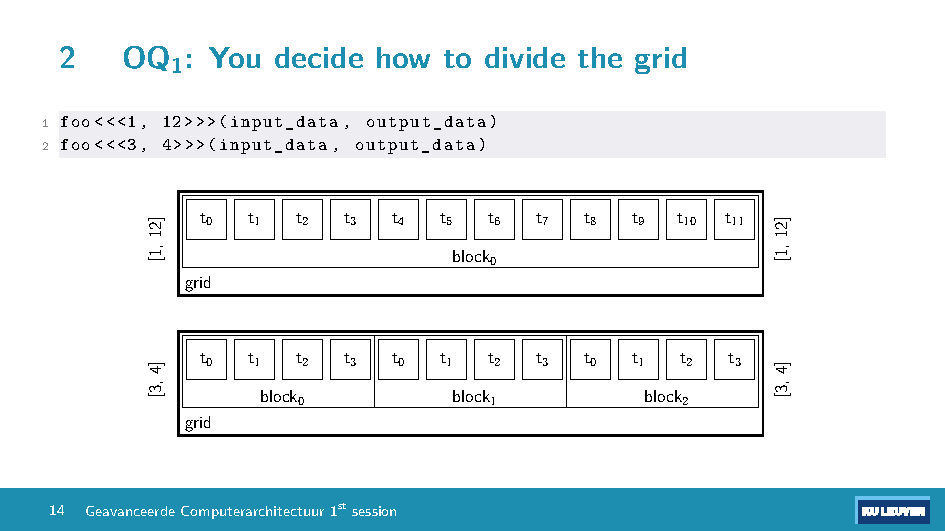
\includegraphics[width=0.72\linewidth, trim=0 20pt 0 0, clip, frame]{figures/session_1_figures/slide-17.pdf}
\caption{You decide how to divide the grid.}
\end{figure}
\begin{figure}[H]
\centering
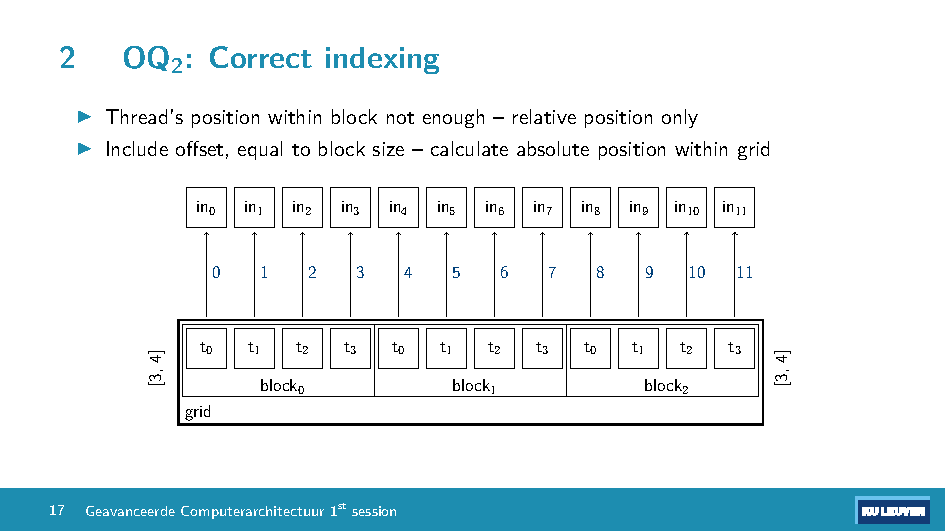
\includegraphics[width=0.72\linewidth, trim=0 20pt 0 0, clip, frame]{figures/session_1_figures/slide-20.pdf}
\caption{Correct indexing: add the block offset to get the absolute position.}
\end{figure}

\subsection{04\_memory.cu}
\paragraph{Short version.}
\begin{lstlisting}[language=CUDA]
// description:  Allocate an array in unified memory, let each GPU thread write its global index into its own element, then print the array on the CPU.

#include <cstdio>
#define N 8

__global__ void fill(int* a){
    int i = blockIdx.x * blockDim.x + threadIdx.x;
    a[i] = i;
}

int main(){
    int* a;
    cudaMallocManaged(&a, N * sizeof(int));
    fill<<<2,4>>>(a);
    cudaDeviceSynchronize();
    for(int i = 0; i < N; i++)printf("%d ", a[i]);
    printf("\n");
    cudaFree(a);
}
\end{lstlisting}
\paragraph{Long version.}
\begin{lstlisting}[language=CUDA]
//  Every line in main() runs on the CPU; only the kernel fill() runs on the GPU.
//   1. int* a;                                   (CPU) Create an empty pointer. It points nowhere yet.
//   2. cudaMallocManaged(&a, N * sizeof(int));   (CPU calls it) Reserve 32 bytes that both CPU and GPU
//                                                can reach, and put the address into a. The memory
//                                                exists now, but holds no useful values yet.
//   3. fill<<<2, 4>>>(a);                        (CPU starts it, GPU runs it) 8 GPU threads each write
//                                                their own index into their own element: 0 1 2 ... 7.
//                                                The CPU does not wait here.
//   4. cudaDeviceSynchronize();                  (CPU) Wait until the GPU has finished filling.
//   5. for loop with printf                      (CPU) Read the array and print 0 1 2 3 4 5 6 7.
//   6. cudaFree(a);                              (CPU calls it) Give the memory back; we are done with it.
#include <cstdio>

// Preprocessor constant: before compiling, every N in the file is replaced by 8.
// It represents the length of the array.
#define N 8

// A kernel that receives a pointer (the address of the array).
// It does not MAKE the array: the memory is reserved in main() by cudaMallocManaged.
// This kernel FILLS the existing array: it writes the values 0..7 into it.
//
// This replaces the CPU loop "for (i = 0; i < N; i++) a[i] = i;" — the threads ARE the loop.
// int* = "pointer to int": a holds a memory ADDRESS, not a number. The kernel needs that address to write into the array that main() allocated. Kernel arguments are copied, but a copied address still points to the same memory, so the writes are visible in main(). A plain "int a" would only be a copy of one number.
__global__ void fill(int* a) {
    int i = blockIdx.x * blockDim.x + threadIdx.x;
    // No bounds check needed HERE because N = 8 and we launch exactly 2 * 4 = 8 threads:
    a[i] = i;
}
int main() {
    // a is a pointer: a variable that holds a memory address (the start of an int array).
    // It does not point anywhere yet.
    int* a;

    // Allocate N * sizeof(int) = 8 * 4 = 32 bytes of unified memory, reachable by both the CPU and the GPU.
    // C++ itself does not guarantee that an int is 4 bytes, which is why you write sizeof(int) instead of 4.
    // & in front of a variable = "address of". a is an int*, so &a is an int** (the address of the pointer itself).
    // cudaMallocManaged has to CHANGE a: it writes the address of the new 32-byte block into it.
    // To change a variable, a function needs that variable's address, so we pass &a, not a.
    cudaMallocManaged(&a, N * sizeof(int));

    // Where is the "int array"? There is no array variable, only:
    //   1. a block of 32 raw bytes, reserved by cudaMallocManaged (bytes have no type)
    //   2. a pointer a that holds the start address of that block
    // The type int* is what makes it an int array: it tells the compiler "at this address are ints of 4 bytes".
    // a[i] is shorthand for *(a + i): start at address a, move i * 4 bytes further, read/write the int there.
    //   a[0] -> byte 0,  a[1] -> byte 4,  a[2] -> byte 8,  ...  a[7] -> byte 28
    // Compare: int b[8]; is a "real" array, but it lives on the CPU stack and the GPU cannot reach it.
    // Memory allocated at runtime (malloc, new, cudaMallocManaged) always comes back as a pointer to its start.

    // a now holds the address of the 32-byte block. We pass a copy of that address to the kernel.
    // The kernel's int* a points to the same memory, so whatever the GPU writes there, main() sees too.
    // No & here: fill does not change a itself, only the memory a points to.
    // No * here: *a would be the value of the first element (an int), not the address of the array.
    fill<<<2, 4>>>(a);

    // The CPU waits until the kernel is done. Only then is it safe to read a on the CPU.
    cudaDeviceSynchronize();

    for (int i = 0; i < N; i++) printf("%d ", a[i]);
    printf("\n");

    // Optional: a (where the array is) and &a (where the variable a itself is) print different addresses:
    // printf("a = %p, &a = %p\n", (void*)a, (void*)&a);

    // Release the memory from cudaMallocManaged (the CUDA equivalent of free()).
    cudaFree(a);
}

// Output:
// 0 1 2 3 4 5 6 7
\end{lstlisting}
\paragraph{Why we need bounds.} The number of threads you launch is always blocks $\times$ threads per block, so it's always a multiple of the block size. The size of your data (N) is set by the problem and almost never matches. The bounds check \texttt{if (i < N)} stops the extra threads from reading or writing memory outside the array. Without it, the program can silently corrupt memory or crash, even when the output looks correct.
\begin{figure}[H]
\centering
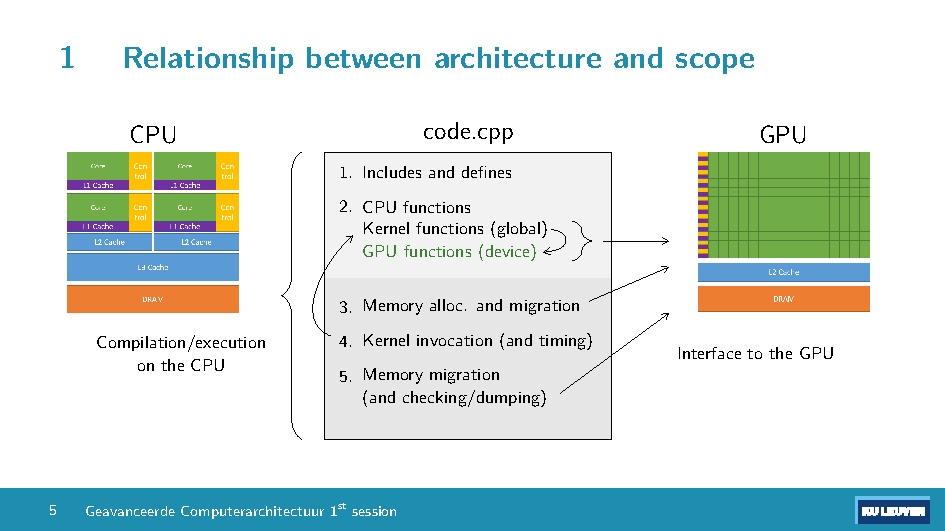
\includegraphics[width=0.72\linewidth, trim=0 20pt 0 0, clip, frame]{figures/session_1_figures/slide-08.pdf}
\caption{Which part of the program runs on the CPU and which on the GPU.}
\end{figure}
\newpage

\subsection{05\_bounds.cu}
\paragraph{Short version.}
\begin{lstlisting}[language=CUDA]
// Description: same exercise as 04, but the number of threads does not equal the number of array elements.
// Fill an array of N = 1000 ints (4000 bytes) on the GPU so that a[i] = i, then print it on the CPU.
// Use 256 threads per block.
// Threads must not write outside the array.

#include <cstdio>

#define N 1000

__global__ void fill(int* a, int n){
    int i = blockIdx.x * blockDim.x + threadIdx.x;
    if(i < n) a[i] = i;
}

int main(){
    int* a;
    cudaMallocManaged(&a, N * sizeof(int));
    int threads = 256;
    int blocks = (N + threads - 1) / threads;
    fill<<<blocks, threads>>>(a, N);
    cudaDeviceSynchronize();
    for(int i = 0; i < N; i++) printf("%d ", a[i]);
    printf("\n");
    cudaFree(a);
}
\end{lstlisting}
\paragraph{Long version.}
\begin{lstlisting}[language=CUDA]
#include <cstdio>

#define N 1000

__global__ void fill(int* a, int n) {
    int i = blockIdx.x * blockDim.x + threadIdx.x;
    // Threads must not write outside the array:
    // 4 blocks * 256 = 1024 threads, but only 1000 elements. Threads 1000..1023 would write past the
    // 4000 allocated bytes. That can corrupt other data, crash, or silently look correct.
    // The bounds check if (i < n) makes those extra threads skip the write.
    if (i < n) a[i] = i;
}
int main() {
    int* a;
    cudaMallocManaged(&a, N * sizeof(int));

    int threads = 256;
    // Integer division rounds DOWN: 1000 / 256 = 3 blocks = 768 threads, which is too few.
    // Adding (threads - 1) makes it round UP: (1000 + 255) / 256 = 4 blocks = 1024 threads.
    int blocks = (N + threads - 1) / threads;
    //  It is the standard integer "ceil": ceil(N / threads) without floats.
    //  Integer division drops everything after the decimal point. Adding threads - 1 (255) pushes any
    //  remainder over the next multiple of 256, but never pushes an exact multiple over:
    //    N = 1000: (1000 + 255) / 256 = 1255 / 256 = 4.90 -> 4   (remainder, so 1 block extra)
    //    N = 1024: (1024 + 255) / 256 = 1279 / 256 = 4.99 -> 4   (exact multiple, no extra block)
    //    N = 1025: (1025 + 255) / 256 = 1280 / 256 = 5.00 -> 5   (1 element left over, 1 block extra)

    // N is the #define above (1000). We pass it to the kernel as parameter n, because the kernel needs the array length for its bounds check.
    // Here the kernel could also use N directly: a #define is not a variable and has no scope; the preprocessor
    // replaces every N with 1000 before compiling. But in real code the length is usually only known at runtime
    // (e.g. read from a file or user input), so it must be passed as a parameter.
    //
    // Why not 1000 blocks of 1 thread? It works, but every block takes at least one warp of 32 threads,
    // so 31 of 32 lanes sit idle, and each SM can only hold a limited number of blocks at once.
    //
    // Why 256 threads? Rule of thumb: a multiple of 32 (the warp size), usually 128 or 256, max 1024.
    // We need one thread per ELEMENT (1000 ints), not per byte (4000 bytes).
    //  a block can have fewer than 32 threads (e.g. <<<1, 8>>>), but the hardware always runs whole warps of 32: the unused lanes are switched off and wasted. That's why block sizes are a multiple of 32.
    fill<<<blocks, threads>>>(a, N);
    cudaDeviceSynchronize();

    for (int i = 0; i < N; i++) printf("%d ", a[i]);
    printf("\n");

    cudaFree(a);
}

// Output (threads 1000 to 1023 exist but write nothing):
// 0 1 2 3 ... 998 999
\end{lstlisting}

\subsection{06\_flip.cu}
\paragraph{Short version.}
\begin{lstlisting}[language=CUDA]
// Description: flip an array on the GPU. Fill an array "in" of N = 9 ints with 0 1 2 ... 8 on the CPU.
// Each GPU thread copies one element of "in" to its mirrored position in a second array "out",
// so that out[N - 1 - i] = in[i]. Print both arrays on the CPU and verify the result.
// Use 4 threads per block. Threads must not read or write outside the arrays.

#include <cstdio>
#define N 9

__global__ void flip(const int* in, int* out, int n){
    int i = blockIdx.x * blockDim.x + threadIdx.x;
    if(i < n) out[n - 1 - i] = in[i];
}

int main(){
    int *in, *out;
    cudaMallocManaged(&in, N * sizeof(int));
    cudaMallocManaged(&out, N * sizeof(int));
    for(int i = 0; i < N; i++) in[i] = i;
    int threads = 4;
    int blocks = (N + threads - 1) / threads;
    flip<<<blocks, threads>>>(in, out, N);
    cudaDeviceSynchronize();
    for(int i = 0; i < N; i++){
        if(out[i] == N - 1 - i) printf("in %d and out %d\n", in[i], out[i]);
        else printf("invalid at %d\n", i);
    }
    cudaFree(in);
    cudaFree(out);
}
\end{lstlisting}
\paragraph{Long version.}
\begin{lstlisting}[language=CUDA]
// Steps in main():
//   1. Reserve two arrays of 9 ints: in and out.
//   2. Fill in on the CPU with 0 ... 8.
//   3. Choose the launch: 4 threads per block, (9 + 3) / 4 = 3 blocks = 12 threads.
//      4 is only to keep the example and its output small; real code uses a multiple of 32 (see 05).
//   4. Launch flip: threads 0..8 each move one element; threads 9..11 are stopped by the bounds check.
//   5. Wait for the GPU.
//   6. Print and verify in one loop: in[i] was i, so out[i] must be N - 1 - i.
//      With a large N you would only print the errors, not every element.
//   7. Free both arrays.
//
// Why two arrays: every thread reads from one array and writes to another, so no thread can
// overwrite a value that another thread still needs. The order in which threads run does not matter.

#include <cstdio>

#define N 9

// in  = pointer to the input array (0 1 2 ... 8). const = the kernel promises to only read it.
// out = pointer to the output array; the kernel writes the flipped values here.
// n   = number of elements (9), needed for the mirror position and the bounds check.
__global__ void flip(const int* in, int* out, int n) {
    int i = blockIdx.x * blockDim.x + threadIdx.x;
    // this is the flipping logic: each thread puts its element at the mirrored position.
    if (i < n) out[n - 1 - i] = in[i];
}

int main() {
    int *in, *out;
    cudaMallocManaged(&in, N * sizeof(int));
    cudaMallocManaged(&out, N * sizeof(int));

    // The starting array is made here: the cudaMallocManaged above reserves the memory,
    // and this loop fills it on the CPU with 0 1 2 ... 8.
    for (int i = 0; i < N; i++) in[i] = i;

    int threads = 4;
    int blocks = (N + threads - 1) / threads; //3
    flip<<<blocks, threads>>>(in, out, N);
    cudaDeviceSynchronize();

    // Print and check in one loop. in[i] was i, so out[i] must be N - 1 - i
    // (the same test as out[N - 1 - i] == i).
    for (int i = 0; i < N; i++) {
        if (out[i] == N - 1 - i) printf("in %d and out %d\n", in[i], out[i]);
        else printf("invalid at %d\n", i);
    }

    cudaFree(in);
    cudaFree(out);
}

// Output:
// in 0 and out 8
// in 1 and out 7
// in 2 and out 6
// in 3 and out 5
// in 4 and out 4
// in 5 and out 3
// in 6 and out 2
// in 7 and out 1
// in 8 and out 0
\end{lstlisting}
\begin{figure}[H]
\centering
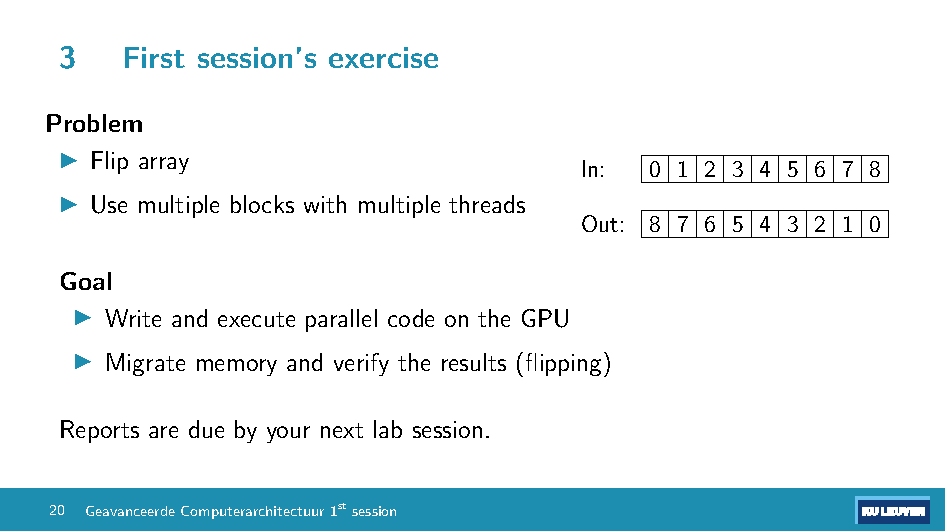
\includegraphics[width=0.72\linewidth, trim=0 20pt 0 0, clip, frame]{figures/session_1_figures/slide-23.pdf}
\caption{First session's exercise: flip an array.}
\end{figure}
\newpage

\subsection{07\_flip\_inplace.cu}
\begin{lstlisting}[language=CUDA]
// Description: same flip as 06, but in place. Use ONE array "a" of N = 9 ints, filled with 0 1 2 ... 8 on the CPU,
// and flip it on the GPU so that it ends as 8 7 6 5 4 3 2 1 0. Print the array on the CPU.
// Use 4 threads per block.
// Avoid a race condition: no element may be written by one thread while another thread reads or writes it.

// In-place is an alternative with one advantage and some drawbacks:
//   + Uses ONE array instead of two: half the memory.
//   - Not faster: both versions read N values and write N values in total.
//   - Easier to get wrong: if all N threads simply copy their element to the mirror position,
//     a thread can overwrite a value that another thread has not read yet (a race condition,
//     topic of session 2). That is why only the first half of the threads work, each swapping one pair.
//   - The original input is gone afterwards, so you cannot compare against it.
// It is included mainly to show a race-condition trap.
//
// What is a race condition?
//   Two or more threads access the SAME memory location, at least one of them WRITES,
//   and nothing controls which one goes first. The result then depends on timing: on which
//   thread happens to be faster. It can be right in one run and wrong in the next.
//   On a GPU, thousands of threads run in parallel in no guaranteed order, so this is easy to cause.
//   Analogy: two people withdraw money from the same account at the same moment. Both read
//   balance 100, both subtract 50, both write back 50. One withdrawal is lost.
//   How to avoid it:
//     - make sure every memory location is written by only one thread (as in 06 and the swap below)
//     - or use synchronization / atomic operations (session 2).
//
// The race condition, concretely. The "obvious" in-place kernel would be:
//
//     if (i < n) a[n - 1 - i] = a[i];      // WRONG: all 9 threads, one array
//
// Thread 0 must write a[0] (= 0) into a[8]. Thread 8 must write a[8] (= 8) into a[0].
// Both touch a[0] and a[8], and nobody decides who goes first:
//   - if thread 8 reads a[8] BEFORE thread 0 overwrites it: a[0] = 8   (correct)
//   - if thread 8 reads a[8] AFTER  thread 0 overwrote it:  a[0] = 0   (wrong: the 8 is lost)
// The same happens for every pair. A possible result is 0 1 2 3 4 3 2 1 0 (a mirror, not a flip),
// and it can differ from run to run. That is what a race condition is: the result depends on
// which thread happens to be faster.
//
// The fix below: only n / 2 threads, and each thread does the WHOLE swap of one pair itself.
// Pair (i, n-1-i) is touched by exactly one thread, so no two threads ever touch the same element.
// tmp is a local variable: every thread has its own private copy (in its own register).

#include <cstdio>

#define N 9

__global__ void flip(int* a, int n) {
    int i = blockIdx.x * blockDim.x + threadIdx.x;
    if (i < n / 2) {
        int tmp = a[i];
        a[i] = a[n - 1 - i];
        a[n - 1 - i] = tmp;
    }
}

int main() {
    int* a;
    cudaMallocManaged(&a, N * sizeof(int));

    for (int i = 0; i < N; i++) a[i] = i;

    int threads = 4;
    int blocks = (N / 2 + threads - 1) / threads;
    flip<<<blocks, threads>>>(a, N);
    cudaDeviceSynchronize();

    for (int i = 0; i < N; i++) printf("%d ", a[i]);
    printf("\n");

    cudaFree(a);
}

// Launch: N / 2 = 4 pairs -> (4 + 3) / 4 = 1 block of 4 threads.
// Thread 0 swaps 0<->8, thread 1 swaps 1<->7, thread 2 swaps 2<->6, thread 3 swaps 3<->5.
// The middle element (4) stays where it is.
// Output:
// 8 7 6 5 4 3 2 1 0
\end{lstlisting}

%=====================================================================
\section{Self-study: practical dim3 examples (2D image, 3D volume)}

Good follow-up practice after \texttt{08\_flip\_2d}. They use the global index from 03 and the bounds check from 05.

\subsection{2D: invert a grayscale image of W $\times$ H pixels}
In memory the image is ONE long array, row after row: pixel \texttt{(x, y)} is at index \texttt{y * W + x}.
\begin{lstlisting}[language=CUDA]
__global__ void invert(unsigned char* img, int W, int H) {
    int x = blockIdx.x * blockDim.x + threadIdx.x;   // column
    int y = blockIdx.y * blockDim.y + threadIdx.y;   // row
    if (x < W && y < H) {
        int i = y * W + x;
        img[i] = 255 - img[i];
    }
}

dim3 threads(16, 16);                         // each block = a 16 x 16 tile of pixels
dim3 blocks((W + 15) / 16, (H + 15) / 16);    // enough tiles to cover the image, rounded up
invert<<<blocks, threads>>>(img, W, H);
\end{lstlisting}
$1920 \times 1080$ image: \texttt{blocks = (120, 68)} $\rightarrow$ $1920 \times 1088$ threads, 1 thread per pixel.
The 8 extra rows of threads are stopped by the bounds check.
In 1D you would launch \texttt{W * H} threads and compute \texttt{x = i \% W}, \texttt{y = i / W} yourself. Same result, less readable.

\subsection{3D: threshold a volume (CT scan, voxel grid) of X $\times$ Y $\times$ Z voxels}
Voxel \texttt{(x, y, z)} is at index \texttt{(z * Y + y) * X + x}.
\begin{lstlisting}[language=CUDA]
__global__ void threshold(float* vol, int X, int Y, int Z, float t) {
    int x = blockIdx.x * blockDim.x + threadIdx.x;
    int y = blockIdx.y * blockDim.y + threadIdx.y;
    int z = blockIdx.z * blockDim.z + threadIdx.z;
    if (x < X && y < Y && z < Z) {
        int i = (z * Y + y) * X + x;
        vol[i] = vol[i] > t ? 1.0f : 0.0f;
    }
}

dim3 threads(8, 8, 8);                                  // each block = an 8 x 8 x 8 cube of voxels (512 threads)
dim3 blocks((X + 7) / 8, (Y + 7) / 8, (Z + 7) / 8);
threshold<<<blocks, threads>>>(vol, X, Y, Z, 0.5f);
\end{lstlisting}

%=====================================================================
\section{Expected for next week}

A \LaTeX-created PDF document with a solution for exercise \texttt{08\_flip\_2d.cu}.

\subsection{08\_flip\_2d.cu: flip a 2D array (mirror an image horizontally)}

\textbf{Problem.} A 2D array of W columns by H rows (think: an image). Reverse every row:

\begin{center}
\begin{tabular}{cc}
\texttt{in:} & \texttt{out:}\\
\begin{tabular}{rrrrrr} 0&1&2&3&4&5\\ 6&7&8&9&10&11 \end{tabular} &
\begin{tabular}{rrrrrr} 5&4&3&2&1&0\\ 11&10&9&8&7&6 \end{tabular}
\end{tabular}
\end{center}

Use a 2D grid of 2D blocks: every thread handles one element and gets an \texttt{x} (column) and a \texttt{y} (row).

\textbf{Goal.}
\begin{itemize}[nosep]
  \item Compute \texttt{x} and \texttt{y} for each thread.
  \item Convert \texttt{(x, y)} to a position in memory.
  \item Bounds check in \textbf{both} directions.
  \item Verify the result on the CPU.
\end{itemize}

%=====================================================================
\section{Lexicon}

\begin{longtable}{@{}p{0.3\linewidth}p{0.66\linewidth}@{}}
\multicolumn{2}{@{}l}{\textbf{Program structure}}\\
\texttt{.cu} file & Source file with CUDA code, compiled with \texttt{nvcc}.\\
\texttt{nvcc} & NVIDIA's CUDA compiler. Splits the code into CPU and GPU parts.\\
host / device & CUDA's names for the CPU and the GPU (used throughout the Programming Guide).\\
kernel & A function that runs on the GPU, launched from the CPU. Marked \texttt{\_\_global\_\_}, returns \texttt{void}.\\
\texttt{\_\_global\_\_} & Marks a kernel: called from the CPU, runs on the GPU.\\
\texttt{\_\_device\_\_} & Marks a helper function that runs on the GPU and can only be called from GPU code.\\
execution space specifier & Keyword that says where a function runs (\texttt{\_\_global\_\_}, \texttt{\_\_device\_\_}, \texttt{\_\_host\_\_}).\\
return type & The type a function gives back (\texttt{void} = nothing). \texttt{main} must return \texttt{int}.\\
scope & The region where a name is visible, e.g.\ a variable inside \texttt{\{ \}} only exists there.\\
\texttt{\#define} / preprocessor & Text replacement before compiling: every \texttt{N} becomes \texttt{1000}. Not a variable, no scope.\\
\noalign{\medskip}
\multicolumn{2}{@{}l}{\textbf{Launching}}\\
launch configuration & \texttt{<<<blocks, threads per block>>>}: how many threads run the kernel.\\
asynchronous & The CPU does not wait after a kernel launch; it continues immediately.\\
\texttt{cudaDeviceSynchronize()} & Makes the CPU wait until the GPU has finished. Also flushes GPU \texttt{printf} output.\\
device \texttt{printf} & The GPU's \texttt{printf}: writes into a buffer in GPU memory, printed at the next sync.\\
\noalign{\medskip}
\multicolumn{2}{@{}l}{\textbf{Thread hierarchy}}\\
thread & One instance of the kernel. Every thread runs the whole kernel body once.\\
block (thread block) & A group of threads (max 1024). Threads in a block run on the same SM.\\
grid & All blocks of one kernel launch.\\
\texttt{threadIdx} & Index of the thread inside its block (\texttt{.x .y .z}). Type \texttt{uint3}.\\
\texttt{blockIdx} & Index of the block inside the grid (\texttt{.x .y .z}). Type \texttt{uint3}.\\
\texttt{blockDim} & Number of threads per block (\texttt{.x .y .z}). Type \texttt{dim3}.\\
\texttt{gridDim} & Number of blocks in the grid (\texttt{.x .y .z}). Type \texttt{dim3}.\\
\texttt{warpSize} & Built-in: number of threads in a warp (32).\\
global index & Unique number per thread over the whole grid: \texttt{blockIdx.x * blockDim.x + threadIdx.x}.\\
\noalign{\medskip}
\multicolumn{2}{@{}l}{\textbf{Hardware}}\\
warp & Group of 32 threads that the hardware always runs together.\\
lane & One of the 32 slots in a warp. Unused lanes are switched off and wasted.\\
SIMT & Single Instruction, Multiple Threads: all threads of a warp execute the same instruction at once.\\
SM & Streaming Multiprocessor: a processing unit of the GPU. Blocks are scheduled onto SMs.\\
occupancy & How many threads/blocks are active on an SM at the same time. Depends on block size, registers and shared memory.\\
register & Fastest memory, private to one thread. Local variables (like \texttt{tmp}) live here.\\
\noalign{\medskip}
\multicolumn{2}{@{}l}{\textbf{Types}}\\
\texttt{struct} & A type that groups several fields, e.g.\ \texttt{x}, \texttt{y}, \texttt{z}.\\
\texttt{dim3} & CUDA built-in vector type: struct with \texttt{x}, \texttt{y}, \texttt{z}. Missing values default to 1.\\
\texttt{uint3} & CUDA built-in vector type: struct with three unsigned ints. Type of \texttt{threadIdx} and \texttt{blockIdx}.\\
\texttt{sizeof(type)} & Number of bytes of a type. \texttt{sizeof(int)} = 4 on all CUDA platforms.\\
\texttt{const} & Promise not to change something. \texttt{const int* in} = the kernel only reads \texttt{in}.\\
\noalign{\medskip}
\multicolumn{2}{@{}l}{\textbf{Memory and pointers}}\\
address & A number that says where something is in memory.\\
pointer (\texttt{int*}) & A variable that holds an address. \texttt{int*} = ``address of an int''.\\
\texttt{\&} (address-of) & \texttt{\&a} = the address of variable \texttt{a}.\\
\texttt{*} (dereference) & \texttt{*a} = the value at the address in \texttt{a}.\\
\texttt{int**} & Pointer to a pointer, e.g.\ \texttt{\&a} when \texttt{a} is an \texttt{int*}.\\
\texttt{a[i]} & Shorthand for \texttt{*(a + i)}: start at \texttt{a}, move \texttt{i} elements further.\\
stack & CPU memory for normal local variables (\texttt{int b[8];}). The GPU cannot reach it.\\
unified memory & Memory that both CPU and GPU can access through the same pointer.\\
\texttt{cudaMallocManaged()} & Allocates unified memory and writes its address into your pointer.\\
\texttt{cudaFree()} & Releases memory from \texttt{cudaMallocManaged} (like \texttt{free()}).\\
row-major & 2D data stored row after row in one array: element \texttt{(x, y)} is at \texttt{y * W + x}.\\
\noalign{\medskip}
\multicolumn{2}{@{}l}{\textbf{Correctness}}\\
bounds check & \texttt{if (i < n)}: stops extra threads from accessing memory outside the array.\\
integer division & Division of ints drops the decimals: \texttt{1000 / 256 = 3}.\\
ceil division & \texttt{(N + threads - 1) / threads}: integer division that rounds up.\\
in-place & Modifying the input array itself instead of writing to a second array.\\
race condition & Several threads access the same memory, at least one writes, and the order is not controlled. The result depends on timing.\\
atomic operation & A read-modify-write that cannot be interrupted by other threads (session 2).\\
synchronization & Making threads wait for each other at a certain point (session 2).\\
\end{longtable}

\end{document}
